\section{Additional results}
\label{sec:S6}

\subsection{Characteristics of the main dataset}
\label{sec:S6.1}

The configuration of the main dataset (ISOMORPH network, flow representation, strain level 75) was selected after a preliminary trial of about forty configurations, on a single criterion, the contrast between policies, without which causal learning would have nothing to identify. The flow representation isolates capacity mechanisms and makes the differences between policies directly interpretable.

The dataset contains 2,000 scenarios, that is, 8,000 crisis versions. The five disruption natures are represented in a balanced way (Table~\ref{tab:d11}). The reference demand, calibrated on the volume that can still be delivered during the incident (Eq.~\eqref{eq:S2}), is very low when the disruption hits the Nashville hub or the Atlanta warehouse, through which the entire flow passes; it reflects the criticality of the affected site as much as the size of the network.

\begin{table}[htbp]
\caption{Characteristics of the main dataset.}
\label{tab:d11}
\footnotesize
\begin{tabularx}{\textwidth}{@{}LL@{}}
\toprule
\textbf{Characteristic} & \textbf{Value} \\
\midrule
Scenarios; crisis versions & 2,000; 8,000 \\
Distribution of natures & Supplier failure 422, storage site closure 405, demand surge 395, congestion 390, link cut 388 \\
Disruption duration, median [quartiles] & 16 days [12; 20] \\
Severity, median [quartiles] & 0.91 [0.82; 0.95] \\
Share of critical items & 0.20 to 0.53 \\
Coefficient of determination, median [quartiles] & 0.88 [0.79; 0.93] \\
Coefficient of determination on smoothed trajectory, median & 0.91 \\
Versions with a drop below 0.03 & 4.2\% \\
Non-finite indicators & 0 \\
Correlation between IPC and observed lost service & 0.97 \\
\bottomrule
\end{tabularx}
\end{table}

The fit is satisfactory for most of the dataset: the median coefficient of determination reaches 0.88 and no indicator is undefined. A quarter of the versions remain below 0.8, mainly short crises or crises with an irregular recovery. The cumulative loss indicator IPC nevertheless remains very faithful to the service actually lost (correlation of 0.97), which justifies making it the main resilience indicator, all the more so as it depends little on shape imperfections of the fitted curve.

\subsection{Effect of the policies by disruption nature and network}
\label{sec:S6.2}

The profiles also differ in the levers they engage: the delayed profile engages only demand levers, as it cannot escalate beyond its first two choices during the crisis; the prudent profile relies mainly on inventories and additional capacity; and the reactive profile on rerouting and capacity. Their effectiveness depends on the nature of the disruption (Table~\ref{tab:d13}).

\begin{table}[htbp]
\caption{Median reduction in cumulative loss relative to no reaction, by disruption nature.}
\label{tab:d13}
\footnotesize
\begin{tabularx}{\textwidth}{@{}LLLL@{}}
\toprule
\textbf{Nature} & \textbf{Reactive} & \textbf{Prudent} & \textbf{Delayed} \\
\midrule
Supplier failure & 84\% & 0\% & 0\% \\
Link cut & 73\% & 17\% & 0\% \\
Storage site closure & 82\% & 10\% & 2\% \\
Demand surge & 87\% & 23\% & 13\% \\
Congestion & 78\% & 41\% & 15\% \\
\bottomrule
\end{tabularx}
\end{table}

The prudent profile has no effect on a supplier failure, which inventory release does not offset, but reduces the loss of a congestion by 41\%, a diffuse disruption that global levers mitigate; the reactive profile is least effective against a link cut, whose effects spread to the backup routes.

To check that these results are not due to the ISOMORPH topology alone, a control batch of 500 scenarios was generated on the parametric network with the same settings. The crises are shallower there (median minimum service level of 0.91) and the fit is poorer, but the cumulative loss remains very faithful to the lost service (correlation of 0.97). The broad proportions are remarkably stable. The share of lost service avoided reaches 67\%, 17\%, and 13\% for the reactive, prudent, and delayed profiles, compared with 73\%, 18\%, and 14\% on ISOMORPH. The topology does, however, change the effectiveness of the levers depending on the nature of the disruption: on the parametric network, whose backup routes have low capacity, the reactive profile reduces the loss of a link cut by only 25\% and that of a closure by only 53\%, compared with 73\% and 82\% on ISOMORPH. The effect of a policy therefore depends jointly on the nature of the disruption and on the redundancy of the network.

\subsection{Prognosis, diagnosis and case study}
\label{sec:S6.3}

Prognosis, based only on the variables known at decision time, correctly classifies 65\% of the test crises, compared with 34\% for the majority class and 60\% for a model based on the policy alone. The gain provided by the context is real but modest. The learning curve is almost flat, from 62.5\% with 200 scenarios to 63.7\% with 1,600. Accuracy is therefore limited by the information available at decision time rather than by the size of the dataset. The loss depends in particular on the strain of the network, which the generator does not export.

Diagnosis is well calibrated for the policy and the duration. For high-loss test crises, the posterior probability of each policy (no reaction, delayed, prudent, reactive) is 0.42, 0.32, 0.26, and 0.01, for observed frequencies of 0.41, 0.33, 0.26, and 0.005; that of a long disruption is 0.41, equal to its observed frequency. It is less well calibrated for the nature of the disruption and the target position, because crises hitting a bottleneck, 6\% of the dataset, are too rare for the score to retain their specific effects.

Two crises of the same nature illustrate the use of the network. In the first, a storage site located on a bottleneck, such as the Atlanta warehouse, is closed for a long time. The network (Figure~\ref{fig:d7}) gives a probability of high loss of 0.70 with no reaction, 0.56 under the delayed profile, 0.44 under the prudent profile, and 0.01 under the reactive profile. Only the latter reaches the objective with sufficient probability, and the recommendation is unambiguous whatever the threshold chosen.

In the second, a redundant storage site is closed for a short time. The probability of high loss falls to 0.30 with no reaction, 0.22 under the delayed profile, and 0.20 under the prudent profile. With $\theta$ = 0.8, the prudent profile reaches the objective with a probability of 0.80 and becomes the recommendation: for a brief disruption on a duplicated site, a reaction based on inventory release is sufficient. Mobilizing rerouting and additional capacity would bring only a marginal gain.

\begin{center}
% Figure: prognosis of the cumulative loss by policy (inference in BayesArtist on the learned network)
% Evidence: nature = fermeture_entrepot, cible = passage_oblige, duree = fort; values read in BayesArtist.
\begin{tikzpicture}[x=1cm,y=1cm, font=\scriptsize]
  \node[anchor=east] at (-0.15,0.00) {Reactive};
  \fill[palmec!75] (0.000,-0.30) rectangle (10.812,0.30);
  \node at (5.406,0.00) {$0.90$};
  \fill[poltard!75] (10.812,-0.30) rectangle (11.904,0.30);
  \node at (11.358,0.00) {$0.09$};
  \fill[polprud!75] (11.904,-0.30) rectangle (11.988,0.30);
  \node[anchor=west] at (12.05,0.00) {$0.01$};
  \node[anchor=east] at (-0.15,-0.90) {Prudent};
  \fill[palmec!75] (0.000,-1.20) rectangle (1.272,-0.60);
  \node at (0.636,-0.90) {$0.11$};
  \fill[poltard!75] (1.272,-1.20) rectangle (6.672,-0.60);
  \node at (3.972,-0.90) {$0.45$};
  \fill[polprud!75] (6.672,-1.20) rectangle (12.000,-0.60);
  \node at (9.336,-0.90) {$0.44$};
  \node[anchor=east] at (-0.15,-1.80) {Delayed};
  \fill[palmec!75] (0.000,-2.10) rectangle (1.056,-1.50);
  \node at (0.528,-1.80) {$0.09$};
  \fill[poltard!75] (1.056,-2.10) rectangle (5.268,-1.50);
  \node at (3.162,-1.80) {$0.35$};
  \fill[polprud!75] (5.268,-2.10) rectangle (12.000,-1.50);
  \node at (8.634,-1.80) {$0.56$};
  \node[anchor=east] at (-0.15,-2.70) {No reaction};
  \fill[palmec!75] (0.000,-3.00) rectangle (0.816,-2.40);
  \node at (0.408,-2.70) {$0.07$};
  \fill[poltard!75] (0.816,-3.00) rectangle (3.600,-2.40);
  \node at (2.208,-2.70) {$0.23$};
  \fill[polprud!75] (3.600,-3.00) rectangle (12.000,-2.40);
  \node at (7.800,-2.70) {$0.70$};
  \draw[black!50] (0,-3.15) -- (12.0,-3.15);
  \foreach \p/\l in {0/0,0.2/0.2,0.4/0.4,0.6/0.6,0.8/0.8,1/1} { \draw[black!50] (\p*12.0,-3.15) -- ++(0,-0.08) node[below] {$\l$}; }
  \node[font=\small] at (6.0,-3.90) {Probability of each IPC cumulative loss class};
  \fill[palmec!75] (1.20,0.55) rectangle (1.55,0.8); \node[anchor=west] at (1.60,0.675) {Low loss};
  \fill[poltard!75] (4.60,0.55) rectangle (4.95,0.8); \node[anchor=west] at (5.00,0.675) {Medium loss};
  \fill[polprud!75] (8.00,0.55) rectangle (8.35,0.8); \node[anchor=west] at (8.40,0.675) {High loss};
\end{tikzpicture}

\captionof{figure}{Prognosis of the cumulative loss by policy, for the long closure of a site located on a bottleneck: distribution of the three IPC classes inferred by the learned network.}\label{fig:d7}
\end{center}

Diagnosis sheds light on the opposite case, a high-loss crisis managed by a prudent profile. The network associates it with a long disruption, with a probability of 0.39 against 0.33 a priori, an almost certain use of inventory release (0.95), and an escalation to three or more levers (0.40 against 0.23 a priori). It thus points to a crisis that is too long for the chosen policy. The operations manager escalated, but starting from inventory levers whose effect wears off, without reaching rerouting in time. This diagnosis directs corrective action toward the policy, which should be more reactive or use a different order of levers, rather than toward the network.

Figure~6 of the main manuscript applies the backward reading of Section~3.4 of the main manuscript to the seven contexts that the ISOMORPH topology makes possible, for the objective of a low cumulative loss. The reactive profile is the most probable everywhere, and more so the longer the disruption lasts: its posterior probability rises from between 0.51 and 0.58 for a short disruption to between 0.72 and 0.79 for a long one. For a short disruption, the three other policies each retain between 0.12 and 0.18: a low loss remains attainable there without a rapid reaction, which is consistent with the sober recommendation of Section~4.3 of the main manuscript. The map, in contrast, varies little with the nature of the disruption and the target position, in line with the diagnosis, since in the learned structure these variables act on the loss only through the levers mobilized.

\subsection{Sensitivity to inventory cover}
\label{sec:S6.4}

The temporal representation makes it possible to study the role of inventories, which the main dataset neutralizes. On the ISOMORPH network, with its original travel times, 60 crises were simulated for each disruption nature and each cover, with no reaction from the operations manager, and we counted those that produce a visible drop in service (Figure~\ref{fig:d8} and Table~\ref{tab:S4}). The flow representation serves as the reference.

\begin{center}
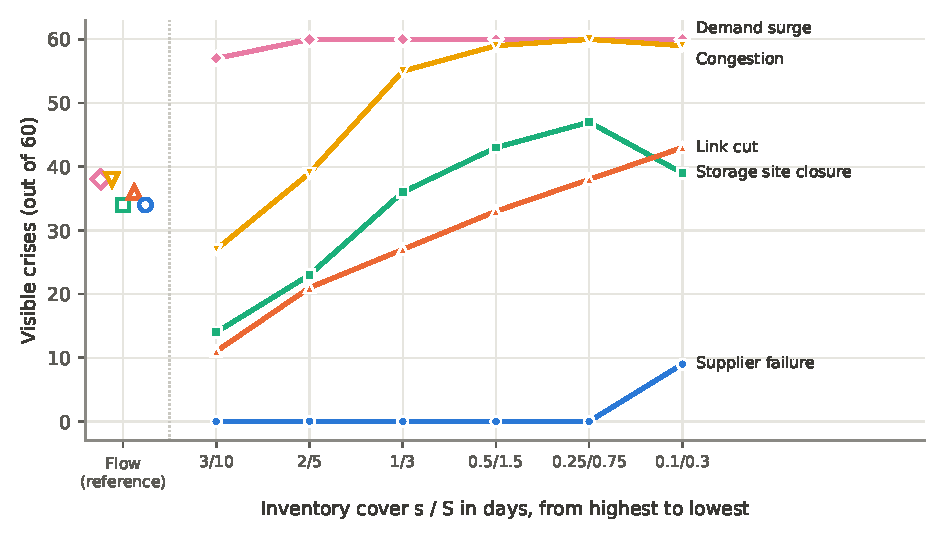
\includegraphics[width=0.75\textwidth]{figures/Fig8_inventory_cover_EN.pdf}
\captionof{figure}{Number of visible crises out of 60 by inventory cover, per disruption nature (ISOMORPH network, no reaction). The hollow symbols on the left give the reference of the flow representation.}\label{fig:d8}
\end{center}

For distribution disruptions (link cut, storage site closure and congestion), inventory cover acts as a gradual robustness lever: the lower it is, the more numerous the visible crises, from 11 to 43 out of 60 for a link cut and from 27 to 59 for a congestion. The boundary between robustness and resilience discussed in Section~S4.3 therefore shifts in a controlled way with the inventory level. Supplier failures, in contrast, are absorbed as soon as the cover reaches a quarter of a day, including failures lasting 15 to 60 days at the default cover: the calibration of demand bounds the shortfall during a failure, which a few days of inventory are enough to offset. Finally, the demand surge is better absorbed without inventories than with them: in the flow representation, any capacity margin instantly serves the additional demand, whereas with lead times this additional demand must first be drawn from inventories sized on the nominal throughput, which replenishment rebuilds only after a delay.

Inventory cover is therefore not a universal resilience lever. It protects against losses of distribution capacity, is almost superfluous against a small upstream failure, and does not protect against a demand shock, which calls for capacity or demand levers. These results, obtained with no reaction from the operations manager and with uniform cover, do not settle the question. The interaction between cover and management policy remains to be studied.

\begin{table}[htbp]
\caption{Crises producing a visible drop in service, out of 60, by inventory cover (ISOMORPH network, no reaction).}
\label{tab:S4}
\footnotesize
\begin{tabularx}{\textwidth}{@{}LLLLLLLL@{}}
\toprule
\textbf{Nature} & \textbf{Flow} & \textbf{3 / 10 d} & \textbf{2 / 5 d} & \textbf{1 / 3 d} & \textbf{0.5 / 1.5 d} & \textbf{0.25 / 0.75 d} & \textbf{0.1 / 0.3 d} \\
\midrule
Supplier failure & 34 & 0 & 0 & 0 & 0 & 0 & 9 \\
Link cut & 36 & 11 & 21 & 27 & 33 & 38 & 43 \\
Storage site closure & 34 & 14 & 23 & 36 & 43 & 47 & 39 \\
Demand surge & 38 & 57 & 60 & 60 & 60 & 60 & 60 \\
Congestion & 38 & 27 & 39 & 55 & 59 & 60 & 59 \\
\bottomrule
\end{tabularx}
\end{table}

\subsection{Detailed economic analysis and cost of overreaction}
\label{sec:S6.5}

The reactive policy is both the most effective and the most profitable per lever: each of its levers preserves on average 6,630 units, or about one third of a day of demand. For a margin of 10 euros per unit, it remains profitable as long as a lever costs less than 66,000 euros per crisis. The prudent policy, in contrast, is economically dominated: it engages more than two thirds of the levers of the reactive policy for a quarter of its gains. Each lever it adds to the delayed policy preserves only 790 units. The cost of a policy therefore depends less on the number of levers than on when they are engaged: engaged early, they prevent the crisis from lengthening; engaged late or in the wrong order, they arrive when most of the loss has already been incurred. Profitability also depends on the nature of the disruption: the break-even ratio of the reactive policy reaches 13,100 units per lever for a supplier failure, but only 2,300 for a congestion, which global levers mitigate poorly. The high break-even ratio of the delayed policy calls for a caveat: its gains come mainly from demand levers, in particular from the postponement of non-critical demand, which raises the measured service level by deferring sales rather than preserving them. Part of these gains is therefore carried over to the following period. Its break-even ratio is probably overestimated.

Figure~7 of the main manuscript draws the consequence for the choice of a policy. Among fixed policies, reactivity is optimal as long as the cost of a lever stays below the break-even ratio of 6,630 units of margin; beyond that, it is better not to react. The prudent and delayed policies are never the best choice. The dashed black curve selects, for each crisis and each lever cost, the policy with the best profit, then averages it over the 2,000 crises. This choice is made a posteriori, as if the outcome of each policy were known in advance: the curve is therefore an upper bound on what a crisis-specific recommendation can yield, of which the Bayesian network, which knows the crisis only partially, captures only a part. This upper bound keeps a positive profit well beyond the break-even ratio of the reactive policy, because for some crises the delayed policy or no reaction is sufficient. For a lever worth 5,000 units of margin, the crisis-specific choice would raise the average profit from 4,560 to 8,350 units per crisis, that is, 83\% more than the best fixed policy; for a more expensive lever, it would remain the only one to yield a gain. The recommendation of the Bayesian network targets precisely this value, by identifying, from what is known about a crisis, the cases where a more sober policy is sufficient.

Two additional batches, with the settings of the main batch, measure the cost of overreaction: 400 scenarios without any perceptible disruption and 300 minor disruptions (severity from 0.1 to 0.3, duration from 1 to 3 days). Without disruption, no profile engages a lever, because detection, based on the smoothed service level, is not triggered by demand fluctuations alone. In the face of a minor disruption, however, the reactive profile engages at least one lever in 32\% of cases, compared with 4\% for the prudent profile and none for the delayed profile, while reducing lost sales only from 2,335 to 2,260 units per crisis. Each lever there preserves about 230 units, nearly thirty times less than over all the crises of the main dataset. The sensitivity of the reactive profile therefore has a real cost in the face of minor disruptions, mostly demand surges and congestions: it is justified only if a minor disruption can be distinguished from a severe crisis, which is what the prognosis of the Bayesian network aims to do.
